
\documentclass{beamer}

\usepackage{algorithm, algorithmic}
\usepackage{amsmath}
\usepackage{caption}
\usepackage{graphicx}

\usepackage[english]{babel}
\usepackage[utf8]{inputenc}
\usepackage[T1]{fontenc}

\usepackage{adjustbox}

\usetheme{metropolis}

\title{\small{Review of\\``Kernel PCA and De-Noising in Feature Spaces''}}
\author{
    Group 7\\
    Henrik Karlsson \texttt{henrik10@kth.se} \and \\
    Alexios Kotsakis \texttt{alexiosk@kth.se}\and \\
    Markus Videll \texttt{mvidell@kth.se}\and \\
    Wenyi Zhao \texttt{wenyizh@kth.se}\and
}
\institute{KTH}
\date{2017-01-16}

\begin{document}

\begin{frame}
    \titlepage
\end{frame}

\begin{frame}
    % The aim of the article - what problem is addressed?
    \frametitle{The Problem}

    % Reconstruction
    % De-noising
\end{frame}


\begin{frame}
    % The Method
    \frametitle{Method}
\end{frame}


\begin{frame}
    \frametitle{Toy Example 1}

\end{frame}

\begin{frame}
    \frametitle{Results for Toy Example 1}
    \begin{figure}
        % 
        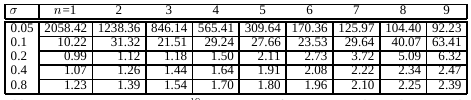
\includegraphics[width=\textwidth]{images/paper-toy1}
        \caption*{Their results for Toy Example 1}
    \end{figure}

    \begin{table}
        \begin{adjustbox}{width=\textwidth}
        \begin{tabular}{c|ccccccccc}
            $\sigma$ & $n=1$ & n=2 & n=3 & n=4 & n=5 & n=6 & n=7 & n=8 & n=9\\
        \hline 0.05 & 919.23 & 538.17 & 341.90 & 226.85 & 132.62 & 108.28 &
        70.69 & 59.65 & 36.25 \\ 0.1 & 240.76 & 136.57 &  72.76 &  51.38 &
        31.60 & 27.90 & 20.39 & 19.83 & 14.20 \\ 0.2 &  47.32 &  29.88 &
        20.12 &  14.62 & 9.60 &   8.57 &  6.75 & 6.07 &  4.71 \\ 0.4 &   8.49
        &   5.72 &   4.26 &   3.02 & 2.22 & 2.05 &  1.49 &  1.72 &  2.02 \\
        0.8 &   1.10 &   0.87 &   0.78 & 0.69 &   0.64 &   0.68 &  0.69 &
            0.73 &  0.76 \\ \hline
        \end{tabular}
        \end{adjustbox}
        \caption*{Our results for Toy Example 1}
    \end{table}
\end{frame}


\begin{frame}
    \frametitle{Toy Example 2}

\end{frame}

\begin{frame}
    \frametitle{Results for Toy Example 2}
    \begin{figure}
        \centering
        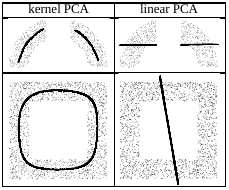
\includegraphics[width=0.35\textwidth]{images/paper-toy2-edit}
        \caption*{Their results for Toy Example 2}
    \end{figure}
    \begin{figure}
        % \centering
            \begin{tabular}{c c c c}
                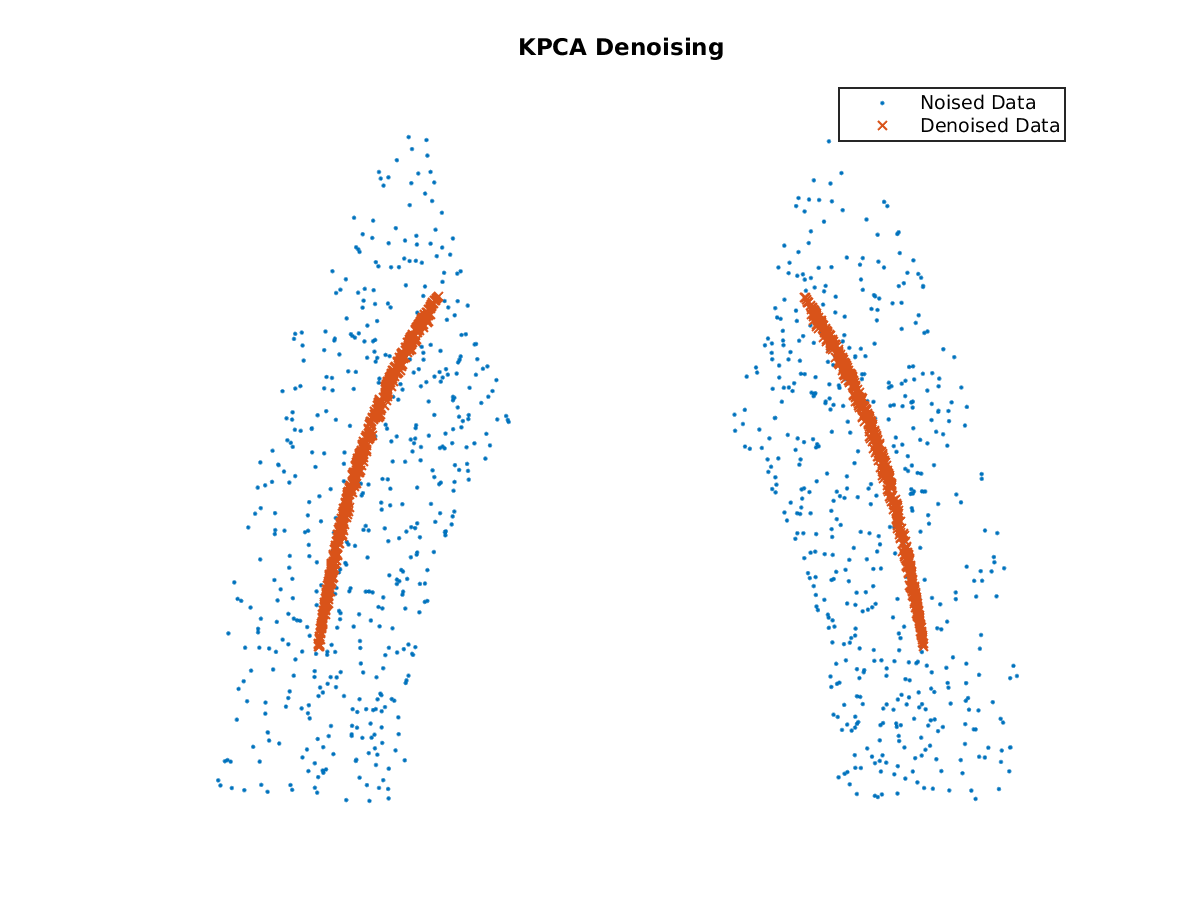
\includegraphics[width=0.20\textwidth]{../code/fig/kpca_circle} &
                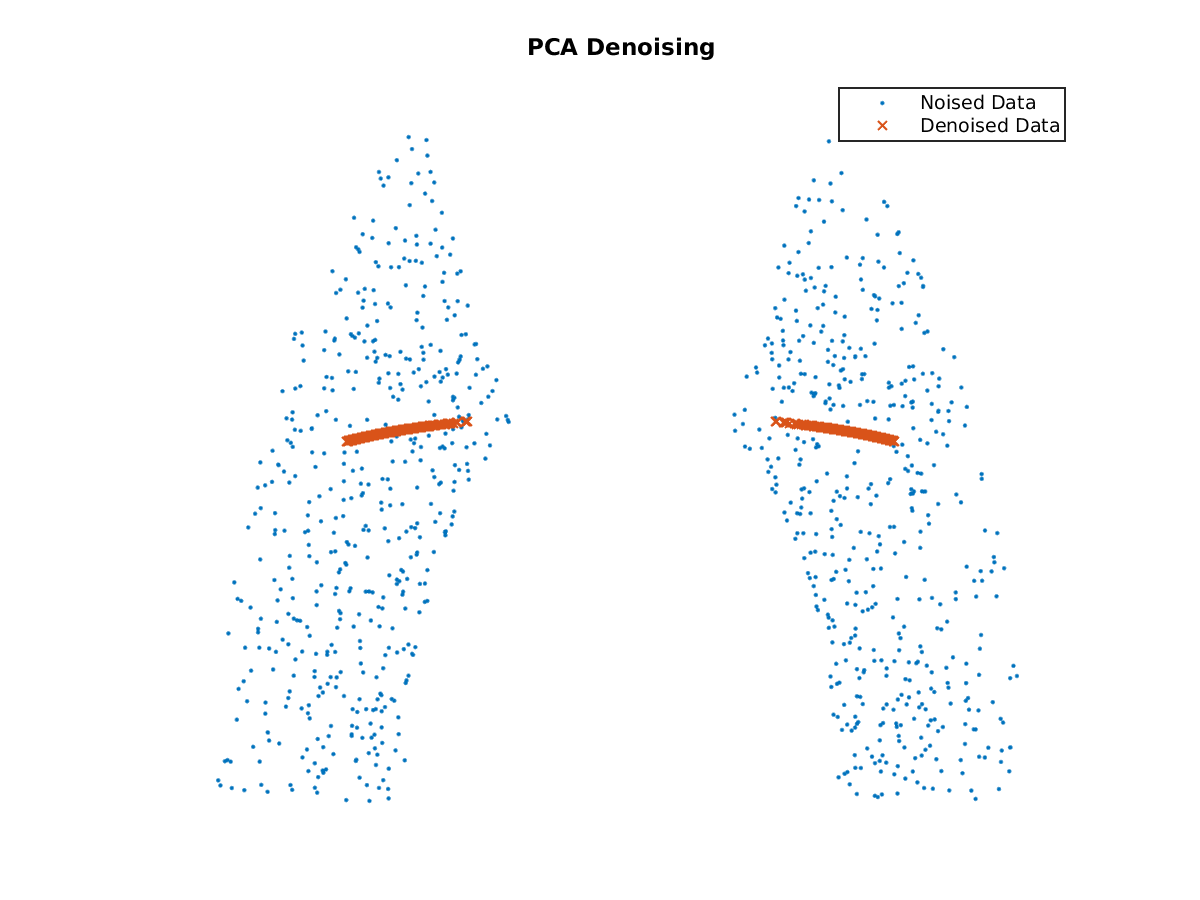
\includegraphics[width=0.20\textwidth]{../code/fig/pca_circle}
                &
                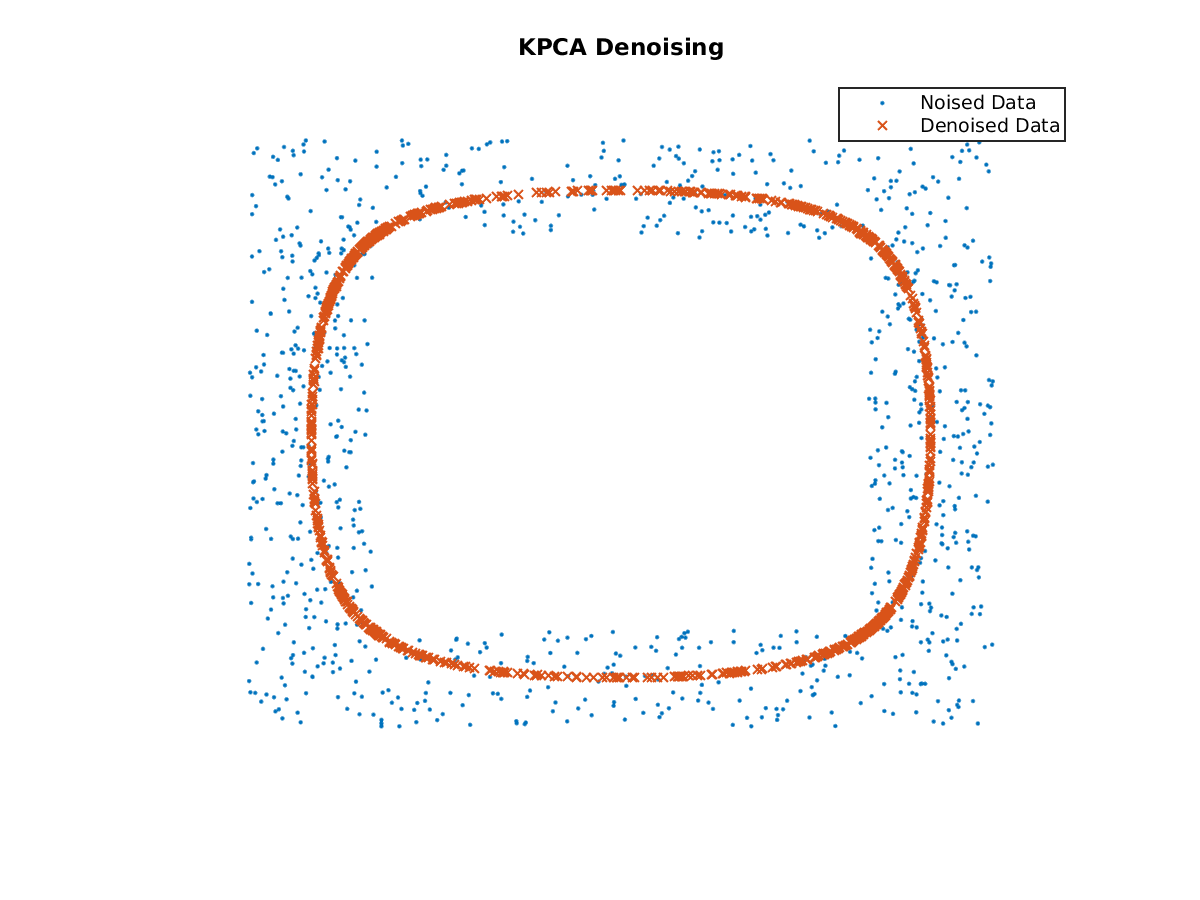
\includegraphics[width=0.20\textwidth]{../code/fig/kpca_box} &
                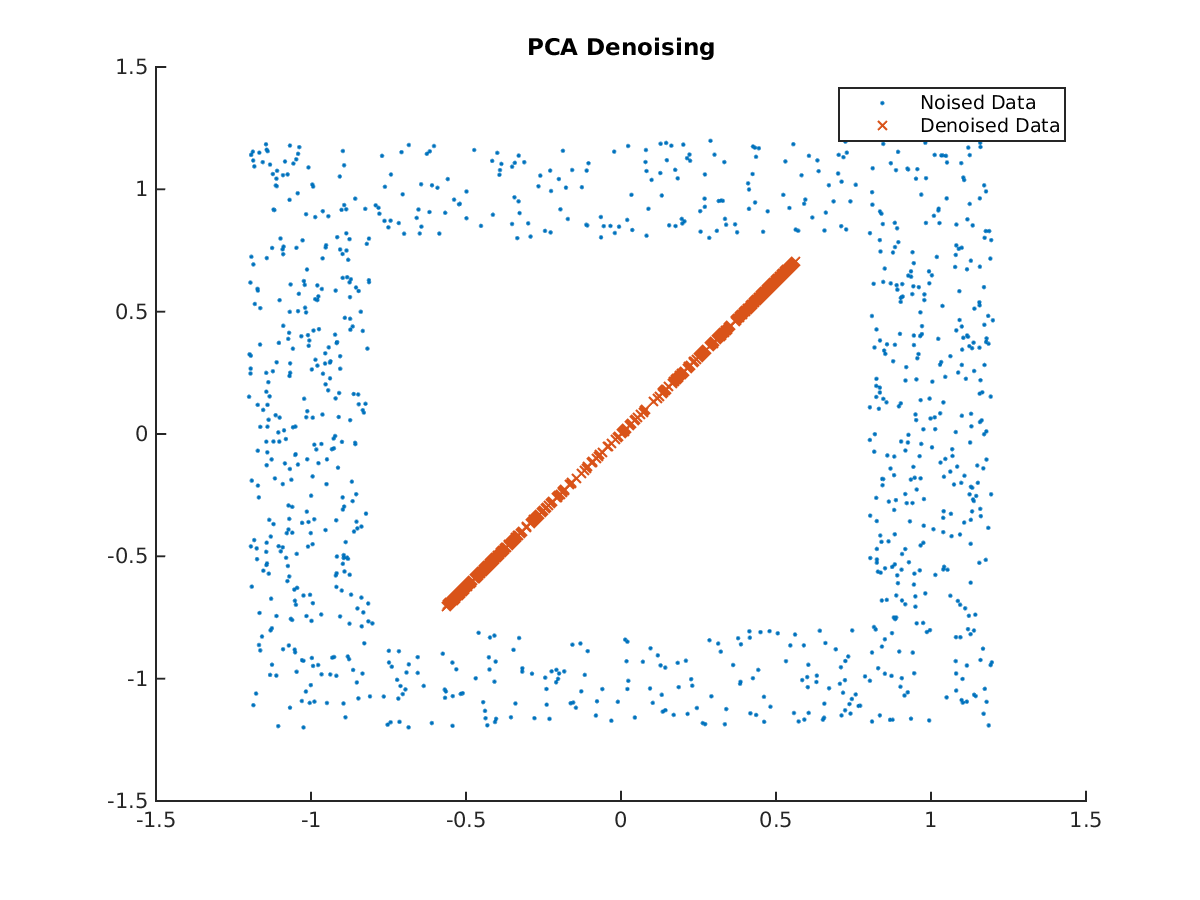
\includegraphics[width=0.20\textwidth]{../code/fig/pca_box} 
            \end{tabular}
        \caption*{Our results for Toy Exmple 2}
    \end{figure}
\end{frame}

\begin{frame}
    \frametitle{USPS Example}
\end{frame}

\begin{frame}
    \frametitle{Results for USPS Example}
    \begin{figure}
    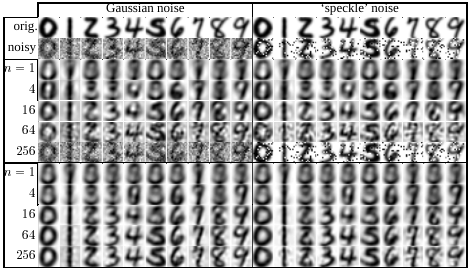
\includegraphics[width=\textwidth]{images/paper-usps}
        \caption*{Their results for USPS dataset}
    \end{figure}

    % Copy the giant table in here
\end{frame}

\begin{frame}
    % If there are differences - what are the reasons?
    % Arguments for and against the method
    \frametitle{Discussion}
\end{frame}

\end{document}


